\section{Hydrogen}

\begin{multicols}{2}


%\section*{}


\subsection{Production of Hydrogen}

\begin{center}
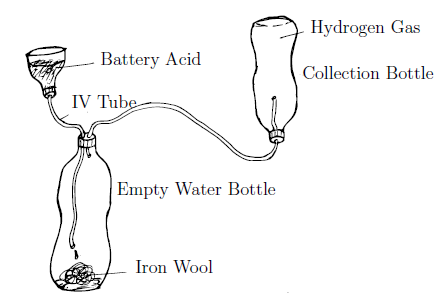
\includegraphics[width=0.4\textwidth]{./img/hydrogen-production.png}
\end{center}

\begin{description*}
%\item[Subtopic:]{}
\item[Materials:]{2 plastic bottles, funnel, iron wool, plastic tube, battery acid}
\item[Setup:]{Poke 2 small holes in a plastic bottle lid. Run 2 plastic tubes (IV tubes/giving sets) through the holes. Connect one to a funnel (cut off bottle) and the other to an empty upturned bottle as shown. }
\item[Procedure:]{Place some iron wool in the bottom of the first bottle and close the lid. Pour battery acid into the funnel so that it falls on the iron wool.}
\item[Hazards:]{Always wear goggles when handling acids.}
%\item[Questions:]{}
\item[Observations:]{Hydrogen gas collects in the upturned bottle.}
%\item[Theory:]{The chemical equation for this reaction is: \[ \mathrm{Fe} + \mathrm{H}_2\mathrm{SO}_4 \longrightarrow \mathrm{Fe}\mathrm{SO}_4 + \mathrm{H}_2 \]}
%\item[Applications:]{}
%\item[Notes:]{}
\end{description*}

\subsection{Hydrogen `Pop'}

%\begin{center}
%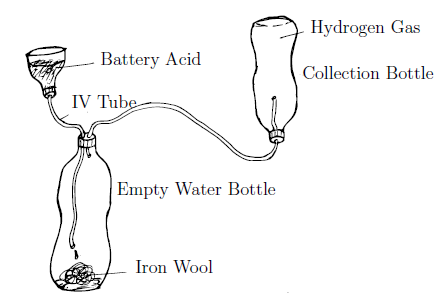
\includegraphics[width=0.4\textwidth]{./img/hydrogen-production.png}
%\end{center}

\begin{description*}
%\item[Subtopic:]{}
\item[Materials:]{Plastic bottle, iron wool, citric acid/battery acid/HCl, funnel, balloon, string, matches, paper}
%\item[Setup:]{}
\item[Procedure:]{Place some steel wool in the bottom of a bottle. Slowly pour the acid into the bottle using a funnel. Stretch a balloon over the mouth of the bottle. After it has inflated, tie the balloon closed with a string and remove from the bottle. Light a long stick or piece of paper and hold it underneath the balloon.}
\item[Hazards:]{HCl burns - wear safety goggles when using it. Do not ignite the balloon near the bottle of acid.}
%\item[Questions:]{}
\item[Observations:]{The balloon fills with hydrogen gas. If using citric acid, it may take longer to fill. When the flame is brought near the balloon, it makes a loud `pop' as it combusts in air.}
%\item[Theory:]{}
%\item[Applications:]{}
\item[Notes:]{You can also use the zinc plate from inside a dry cell in place of iron wool.}
\end{description*}

\columnbreak

\subsection{Hydrogen Bubbles}

\begin{center}
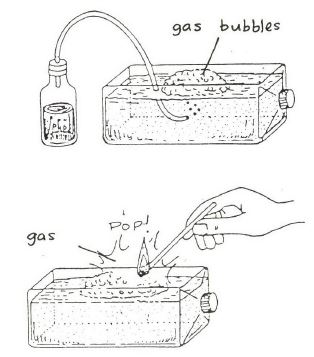
\includegraphics[width=0.4\textwidth]{./img/source/hydrogen-bubbles.jpg}
\end{center}

\begin{description*}
%\item[Subtopic:]{}
%\item[Materials:]{}
%\item[Setup:]{}
\item[Procedure:]{Produce hydrogen gas as described above, but run the tube into a water bath. When you begin to see bubbles being produced, bring a long lit stick or burning paper near the bubbles and hear the loud `pop.'}
%\item[Hazards:]{}
%\item[Questions:]{}
%\item[Observations:]{}
%\item[Theory:]{}
%\item[Applications:]{}
%\item[Notes:]{}
\end{description*}

%==================================================================================================%


\end{multicols}

\pagebreak